\documentclass[a4paper,11pt,dvipdfmx]{ujarticle}
% パッケージ
\usepackage{graphicx}
\usepackage{url}
% レイアウト指定を記述したファイルの読み込み
\input{layout}

% タイトルと氏名を変更せよ．
\title{日本におけるデジタル化の状況}
\author{金子 優}

\begin{document}

\maketitle %タイトル
\section{ブロードバンドの整備状況}
OECDによるブロードバンド回線の普及に関する調査\cite{oecd}によると、図\ref{a}に示すように、日本における100人あたりの光ファイバー回線の加入者は29.0で韓国、スウェーデン、ノルウェーに続いて第４位になっている。
\begin{figure}[htbp]
    \centering
    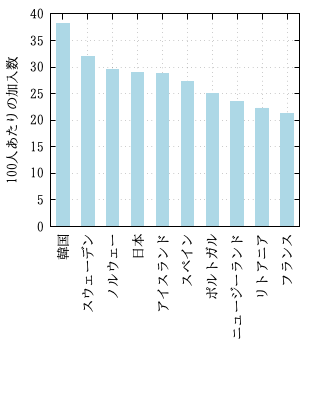
\includegraphics{fig11.png}
    \caption{光ファイバー回線の加入者数(100人あたり)}\label{a}
\end{figure}
\section{デジタル競争力ランキング}
国際経営開発研究所(IMD)の調査\cite{imd}によると、日本のデジタル競争力のランキングは表\ref{b}に示すように、調査対象の64カ国中、総合で28位、技術分野で30位となっている。
\begin{table}[htbp]
    \centering
    \caption{デジタル競争力ランキング(64カ国中)}\label{b}
    \begin{tabular}{|c|c|c|}
        \hline
        国 & 総合 & 技術 \\
        \hline
        米国 & １位 & 4位 \\
        \hline
        香港 & ２位 & 10位 \\
        \hline
        スウェーデン & ３位 & 8位 \\
        \hline
        デンマーク & 4位 & 2位 \\
        \hline
        シンガポール & ５位 & 3位 \\
        \hline
        \hline
        韓国 & 12位 & 13位 \\
        \hline
        中国 & 15位 & 20位 \\
        \hline
        \hline
        日本 & 28位 & 30位 \\
        \hline

        
    \end{tabular}

\end{table}
\section{考察}
\begin{itemize}
    \item 日本における光ファイバー回線は世界的に見ても高水準であると考えられる。
    \item 人材不足なので育成を急がなければランキングは上がらないと考えられる。
\end{itemize}
 
%ここから本文
% 節見出し: \section{}
% を使う
% 本文(1)
%  参考文献の参照: \cite{}
%  図番号の参照： \ref{}
% を使う
% 文献データベースのキーワードは oecd と imd
% になっている．

% 図の挿入
% \includegraphics{}
% を
% \begin{figure}[htbp]
% \end{figure}
% で囲み
% \caption{}
% で図のタイトルを入れる．
% \label{}
% を使って図番号が参照できるようにする
% また，
% \centering
% で図が中央に来るようにする

% ーーー
% 節見出し(2)

% 本文(2)

% 表の挿入
% \begin{tabular}
% \end{tabular}    
% による表の記述を 
% \begin{table}[htbp]
% \end{table}
% で囲み
% \caption{}
% で表のタイトルを入れる．
% \label{}
% を使って表番号が参照できるようにする
% また，
% \centering
% で表が中央に来るようにする

% ーーー
% 見出し(3)
% 考察
%
% \begin{itemize}
% \end{itemize}
% を使って箇条書きで記述する

% ここに参考文献が入る
%
\bibliographystyle{junsrt}
\bibliography{exercise.bib}

\end{document}